\documentclass{beamer}

\usepackage[utf8]{inputenc}

\title{Coding Goûter}
\author{Zeste de Savoir}
\usetheme{zestedesavoir}
\begin{document}

\begin{frame}
  \titlepage
\end{frame}

\section{Association ZDS}

\begin{frame}
  \frametitle{Présentation de Zeste de Savoir}
  \begin{center}
        
\includegraphics[width=10cm]{zds.png}
    \end{center}
\end{frame}

\begin{frame}
    \frametitle{Présentation de Zeste de Savoir}
    Objectif de l'association : Promouvoir le partage de connaissances et d’aider à l’auto-formation dans divers domaines, notamment informatiques et scientifiques.
\end{frame}

\begin{frame}
    \frametitle{Présentation de Zeste de Savoir}
    \begin{center}
        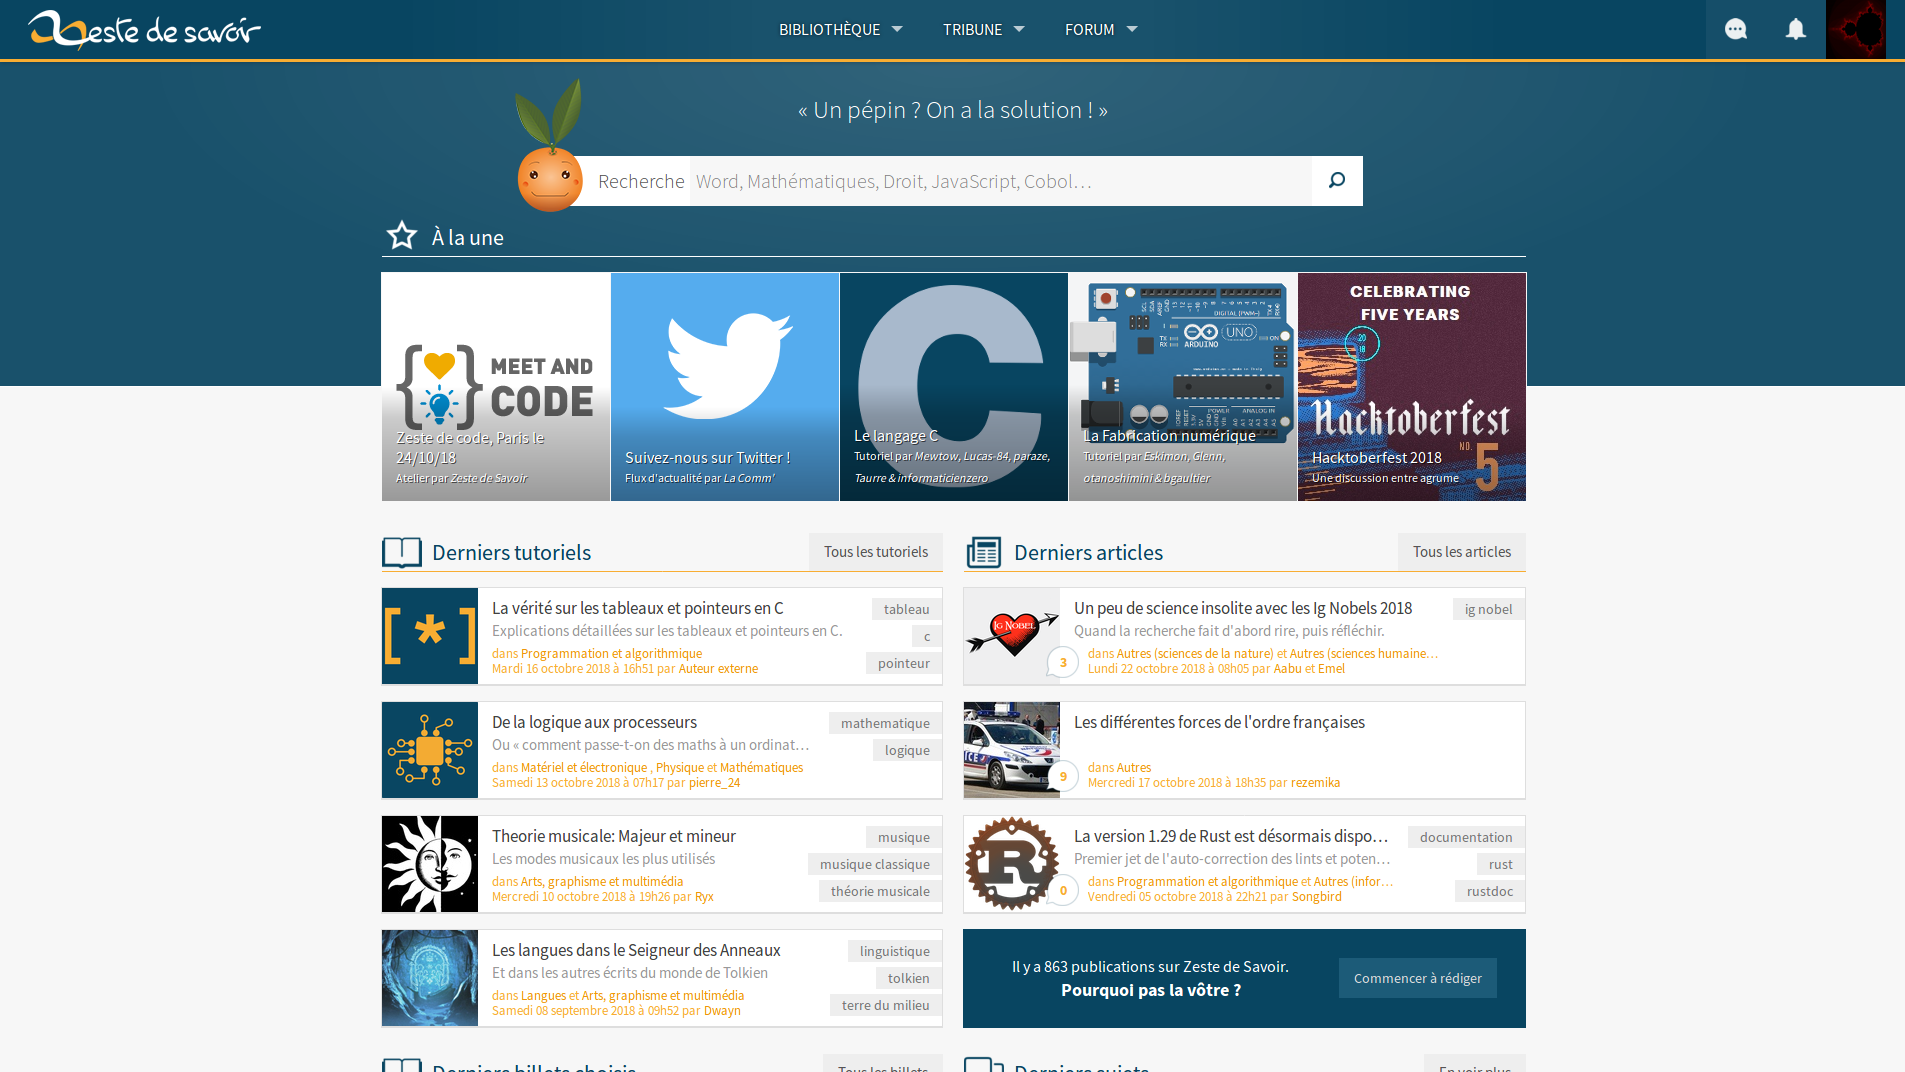
\includegraphics[width=10cm]{captureZDS.png}
    \end{center}
\end{frame}

\begin{frame}
    \frametitle{Présentation de Zeste de Savoir}
    Quelques savoirs sur notre site :
    \begin{itemize}
        \item Musique : théorie musicale, débuter avec le jazz, la physique des cordes de guitare
        \item Le système électoral
        \item Électronique : Arduino, premiers pas dans l'informatique embarquée
        \item Informatique : Apprendre à programmer avec Python
    \end{itemize}
    Plusieurs formats : forum, article, tutoriel, tribune libre.
\end{frame}

\section{Atelier Meet\&Code}

\begin{frame}
    \frametitle{Meet\&Code}
    Semaine européenne du code : du 6 au 21 octobre 2018.
    \\(avec un peu de retard)
    \begin{center}
        
\includegraphics[width=4cm]{meetandcode.png}
        \\Meet\&Code finance cet évènement
    \end{center}
\end{frame}

\begin{frame}
    \frametitle{Que veut dire programmer ?}
    Programmer (= coder) :
    \begin{itemize}
    \item Écrire un programme informatique
    \item Établir à l'avance une suite d'opérations ; planifier.
    \end{itemize}

    Programme (= code) : Description de la suite d'opérations que doit effectuer une machine.
\end{frame}

\begin{frame}
    \frametitle{Que veut dire programmer ?}
    Concrètement, parler à l'ordinateur pour lui dire quoi faire.

    Analogie avec la recette de cuisine :
    \begin{itemize}
        \item Casse 4 oeufs dans un saladier
        \item Ajoute 150g de farine, 150g de sucre et 150g de beurre
        \item Ajoute une pincée de sel et un paquet de levure
        \item Mélange avec un fouet pendant 2 minutes
        \item Enfourne thermostat 7 pendant 10 minutes
    \end{itemize}
\end{frame}

\begin{frame}
    \frametitle{Quelle langue pour parler à l'ordinateur ?}
    \begin{itemize}
        \item Langues que l'humain parle : français, anglais...
        \item Langue que l'ordinateur parle : binaire (001010101101)
    \end{itemize}

    Solution : faire une langue intermédiaire
    \begin{itemize}
        \item Python
        \item Scratch
    \end{itemize}
\end{frame}

\begin{frame}
    \frametitle{Pourquoi programmer ?}
    \begin{itemize}
        \item Mieux comprendre le fonctionnement des ordinateurs
        \item Créer des programmes
        \item S'amuser
    \end{itemize}
\end{frame}

\end{document}